\documentclass[preprint2,numberedappendix,tighten,twocolappendix]{aastex6}
\shorttitle{ECHO}
\shortauthors{Jacobs, et. al.}

\usepackage{amsmath}
\usepackage{graphicx}
\usepackage[figuresright]{rotating}
\usepackage{natbib}
\usepackage{ctable}
\usepackage{tabularx}
\usepackage{enumitem}
\usepackage{url}
\setlist[itemize]{noitemsep, topsep=0pt}
\setlist[enumerate]{noitemsep, topsep=0pt}
\citestyle{aa}

%\AuthorCallLimit=2

\begin{document}


\title{The External Calibrator for Hydrogen Observatories}



\author{
Daniel C. Jacobs\altaffilmark{1},
Jacob Burba\altaffilmark{2},
Judd Bowman\altaffilmark{1},
Lauren Turner\altaffilmark{1},
Benjamin Stinnett
}

\altaffiltext{1}{School of Earth and Space Exploration, Arizona State U., Tempe, AZ, 85287}
\altaffiltext{2}{Brown University, Providence, RI}


\begin{abstract}
Multiple instruments are pursuing constraints on dark energy, observing reionization and opening a window on the dark ages through the detection and characterization of the 21cm hydrogen line across the redshift spectrum, from nearby to z=25.  These instruments including CHIME in the sub meter and HERA in the meter bands are wide-field arrays with multiple degree wide beams operating in transit mode.  Accurate knowledge of the primary beam is critical for separation of bright foregrounds motivating investigation into the use of autonomous drones.  Previous work has focused on model verification and does not address the need of 21cm experiments for routine beam mapping, to the horizon, of the as-built array.  Here we describe the design and methodology of a drone mounted calibrator, the External Calibrator for Hydrogen Observatories (ECHO) which aims to address this need. We report on a first set of trials matching the ECHO measurements against other calibration methods.  These experiments find a worst-case error of 2\% which is about double the requirement and suggest that the desired precision and angular coverage is achievable in practice. We identify the main sources of error and describe steps needed to overcome them.
\end{abstract}




\section{Introduction}\label{sec:intro}

A new generation of radio arrays is being developed that use large numbers of low-cost elements, such as phased tiles of dipole antennas. This is made possible by developments in digital technology and enables exploration of new windows on the universe such as the epoch of reionization (EoR) via the redshifted 21 cm line \citep{Morales:2010p8093,Furlanetto:2006p2267,Madau:1997p2232}. Precise calibration of the primary beams of these dipole arrays has been found to be crucial to analysis of observations by widefield radio arrays such as the MWA \citep{Tingay:2013p9022,Bowman:2013p9950}, PAPER \citep{Pober:2012p8800,2015ApJ...809...61A,2013ApJ...776..108J}, LOFAR \cite{Yatawatta:2013p9699}, HERA \citep{2016:deBoerHERAarxiv} and SKA-low \citep{Mellema:2013p10035,Mort:2016SKAlowimagingarxiv}.

The chief challenge in observing highly redshifted 21\,cm is discriminating the mK level spectral line signal against the $\sim$100K foregrounds.  Instrumental simulations have found that bright sources far from the pointing center, though attenuated significantly by the beam, introduce foreground signals which are highly chromatic and difficult to discriminate from the cosmological 21cm spectral line signature \citep{Thyagarajan:2013p10039,2015ApJ...804...14T,Mort:2016SKAlowimagingarxiv}. These effects have been confirmed in both MWA and PAPER observations \citep{2015:ThyagarajanConfirmationwidefield,Pober:2016ApJ...819....8P}. Precision removal of foreground sources far into the sidelobes is one of the chief challenges of the primary analysis pipelines  \citep{2016:JacobsPipelinepaper} however the amount which can be removed is limited by the accuracy of our knowledge of the antenna response.  More detailed electromagnetic models have been shown to improve the overall accuracy of flux reconstruction \citep{Sutinjo:2015RaSc...50...52S}. however a single digital model cannot account for as-built variation which has been shown to be significant and largely unavoidable without large added expense \citep{2016:NebenBeamformingerrors}.  The largest success of improved modeling accuracy has been in improving polarization response. Polarization signals have inherent spectral variation due to faraday rotation imprinted by magnetized ionized plasmas in the interstellar medium as well as the ionosphere. Leakage of these spectral signatures into the unpolarized reionization signal can be minimized with a combination of beam modeling and careful element design \citep{Jelic:2010p8293,Moore:2013p9941,Asad:2015LofarPol}.
\begin{figure*}[hbt]
\centering
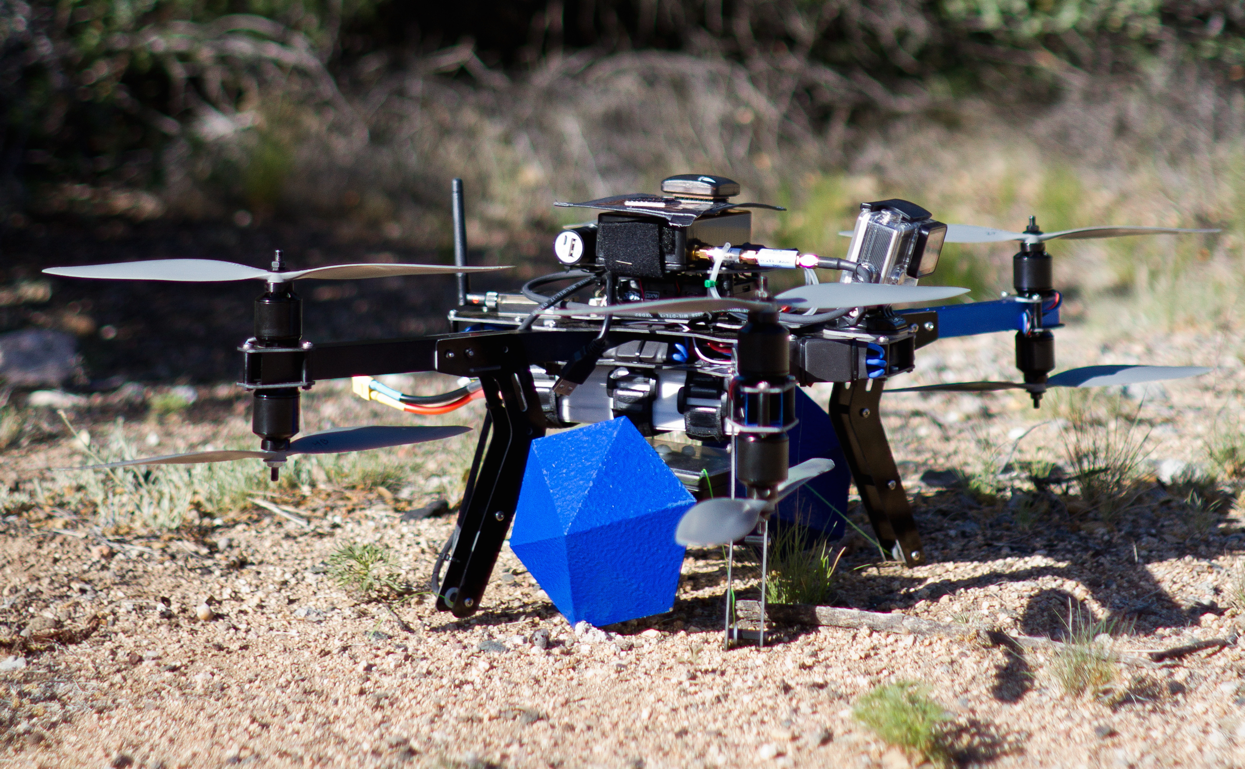
\includegraphics[width=0.59\textwidth]{figures/drone2.png}
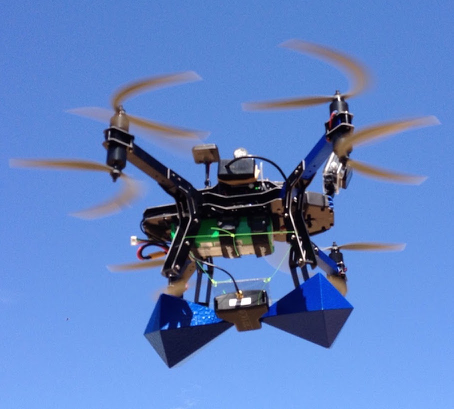
\includegraphics[width=0.4\textwidth]{figures/drone.png}
\caption{3DR X8 octoquad drone prior to launch (left) and in flight (right).  The transmitter is contained in the black project box mounted on top of the drone.  A copper plate, which acts as shielding from the electronics below, with the attached GPS/magnetometer attached atop the project box. Beneath the drone, the blue  BicoLOG antenna is slung with non-conductive monofilament. For scale note that props are 30cm tip to tip and the antenna cone is 10cm at its widest point.}
\label{fig:drone}
\end{figure*}
Another feature of 21cm observations is the wide spectral bandwidth, at least 100 to 200 MHz to span a useful redshift range. Successful foreground isolation across this range necessitates knowledge of the beam response across this entire range.  Spectral variation of the beam has been found to cause otherwise smooth foregrounds to contribute an additional foreground component\citep{2016:ThyagarajanBeamChromaticity,2016:EwallWiceHERAdisharXiv}. An inaccurate beam model also limits the accuracy of calibration. The usual solution is to only use calibration sources in the well known parts of the beam, however incomplete foreground models have been shown to lead to spectral line foregrounds \citep{2016:BarryCalibrationRequirements}.  Calibration error is not just limited to sky modeling. Arrays such as PAPER and HERA are taking advantage of baseline redundancy to calibrate without sky models \citep{Liu:2010p10391,Zheng:2014p10467,2015ApJ...809...61A}, however this technique is subject to error due to deviations from redundancy caused by beam variation from antenna to antenna. Though more work is necessary to understand the impact of beam non-redundancy, its clear that more needs to be known about the actual as-built variation.  Accurate knowledge of the beam can dramatically improve the quality of analysis steps but is also key information during the design process as a validation of modeling and to explore design choices \citep{2014IAWPL..13..169V,2016:NebenHERAdish}. 

While instrument modeling and pipeline development results all agree that accurate beam characterization is critical, there is little certainty as to a specific requirement on that accuracy.  \citet{Shaw2015_chimemmodes} have placed a requirement of 0.1\% accuracy on the width of the beam for the CHIME experiment. This is roughly in agreement with the suggestion within the HERA collaboration that 1dB standard deviation at the -40dB beam level is a good goal.

Taken together, we can summarize the 21\,cm needs for beam measurements as:
\begin{itemize}
\item maps of the in-situ / as-built antennas
\item precision at the horizon as good as the phase center (1dB at -40dB)
\item sampling across the desired bandwidth
\item full polarization sampling
\end{itemize} 




Beam calibration of low frequency dipole arrays poses several complications compared to traditional dish antennas. Most notable is that traditional beam calibration, where the beam is scanned across a bright isolated source, is not possible because arrays are fixed to the earth. Phased array beams are technically steerable but violate the assumption that the beam is constant as it scans. Drift scan calibration of dipole array beams is possible --tracking point sources as they track across the beam--- but it requires the test antenna/array to be embedded within an existing array that generates sufficient sensitivity to isolate a large number of radio sources to provide many tracks through the beam or availability of a large steerable dish with which to cross-correlate\citet{Berger:CHIME_beam_map2016-arxiv}. Even if source tracks can be measured at high sensitivity there is still the issue that sky sources only measure parallel cuts along one direction and cannot as easily constrain the beam along the declination direction. \citet{Pober:2013p9942} have employed symmetry arguments to tie the different right ascension tracks together, but this is not possible in general for more complicated dipole array beam patterns and is ultimately limited by the symmetry argument and in the sensitivity far out in the beam.   Attempts have been made to use anechoic chambers to calibrate low-frequency phased arrays, but the measurements suffer since even the largest chambers cannot extend into the farfield pattern and the RF absorber material used in the chambers performs poorly below 150 MHz, creating reflections and resonances and in any case does not capture the as-built variation. Mapping beam response using the Orbcomm constellation of satellites has proven the most effective \citep{2015RaSc...50..614N,2016:NebenHERAdish} but is limited to only a single frequency (138 MHz).  


Measurement using a nearby emission source must take into account near-field effects. Airborne calibrators are particularly well suited to instruments with a reachable far-field distance. 
%TODO need a cite for this
The far field is defined as the distance at which wavefronts are approximately planar across the element in question, an approximate definition is the square of the aperture size over the wavelength. Table \ref{tab:table} gives a list for a few representative 21cm arrays. The far field for HERA is 100m, which is a reasonable operating hight for a small drone.  However, we should note that it is possible to translate near field  measurements into the far-field by measuring maps at multiple distances, as is commonly done in the laboratory calibration of optical and millimeter instruments.

\begin{deluxetable}{cccc}
\tablecaption{Far field distances for m and subm telescopes \label{tab:table}}
\tablehead{
\colhead{Element} & \colhead{Aperture Diameter} & \colhead{Wavelength} & \colhead{Far field} \\
\colhead{} & \colhead{m} & \colhead{m} & \colhead{m}\\
}
\startdata
PAPER & 2 & 2 & 2\\
MWA  & 5 & 2 & 12.5\\
HERA & 14 & 2 & 98 \\
LOFAR & 41 & 2 & 840.5\\
CHIME & 20 & 0.1 &  4000 \\  
HYRAX & 12 & 0.1 & 1,440 \\ %hirax is just an estimate
VLA & 25 & 0.2 & 2,970\\
\enddata
\end{deluxetable}



 Drone-based radio calibration has recently been explored for application to widefield 21cm instruments. A drone-mounted calibration source was used to verify the accuracy of antenna response modeling for SKA-low stations \cite{2014IAWPL..13..169V} and then a second generation setup was then used as a phase calibrator \citep{2015ExA....39..405P}.  Fully mapping the beam of an antenna has been demonstrated by \citet{2015PASP..127.1131C}.  In that experiment, a 5m dish was mapped at 1GHz with a noise source broadcast by a gimbal mounted horn. This experiment provided a first demonstration of the drone beam-mapping concept and identified places for improvement of the methods.   

Future improvement areas included: optimizing the flight path to better sample the beam, obtaining better drone positioning accuracy, improving characterization of the transmitter beam, and better modeling of the antenna under test. This last point was partially motivated by a lack of alternate beam mapping data with which to compare the results. Additional changes must be made in the shift from low redshift intensity mapping applications at 1GHz to reionization and cosmic dawn 200MHz.  At these lower frequencies horns and other highly directive elements become prohibitively large and heavy for flight applications, motivating the use of a fixed dipole, such as was used by \citet{2014IAWPL..13..169V}, while the broader effective bandwidths and heavier power amplifiers make coverage of the entire band add additional weight. The use of a fixed dipole puts further emphasis on the need to better understand the transmitter beam pattern with modeling and alternate measurements. 


In this paper we report our progress towards overcoming these challenges with the development of the External Calibrator for Hydrogen Observatories (ECHO) which adds to previous development efforts and specifically addresses the 21\,cm requirements identified above.  The ECHO system described in section \ref{sec:design} uses a broadband dipole mounted in a fixed way beneath a multi-rotor drone. The antenna is driven by a sine-wave source which provides suitable power at a fixed frequency. Beam maps are captured by flying the transmitter in a grid over the antenna using a novel application of a well-known spherical mapping pattern.  As a test of the method section \ref{sec:orbcomm} describes how we have mapped two calibration dipoles which also serve as calibrators when using commercial satellites as beam mapping sources.  Comparing our measurements with the satellite data and with simulations we can quantify the measurement stability and overall accuracy.  In section \ref{sec:conclusion} we summarize the conclusions from these tests and identify places for further improvement



%  In section \ref{sec:design}, we describe our drone and transmitter design, improved flight procedure and analysis method.  In section \ref{sec:orbcomm} we detail the results of mapping the reference dipoles used in the Orbcomm mapping setup which lets us compare with both detailed models and measured beam response maps.  Section \ref{sec:conclusion} summarizes the results so far and outlines the next steps.


\begin{figure*}[htb]
\begin{center}
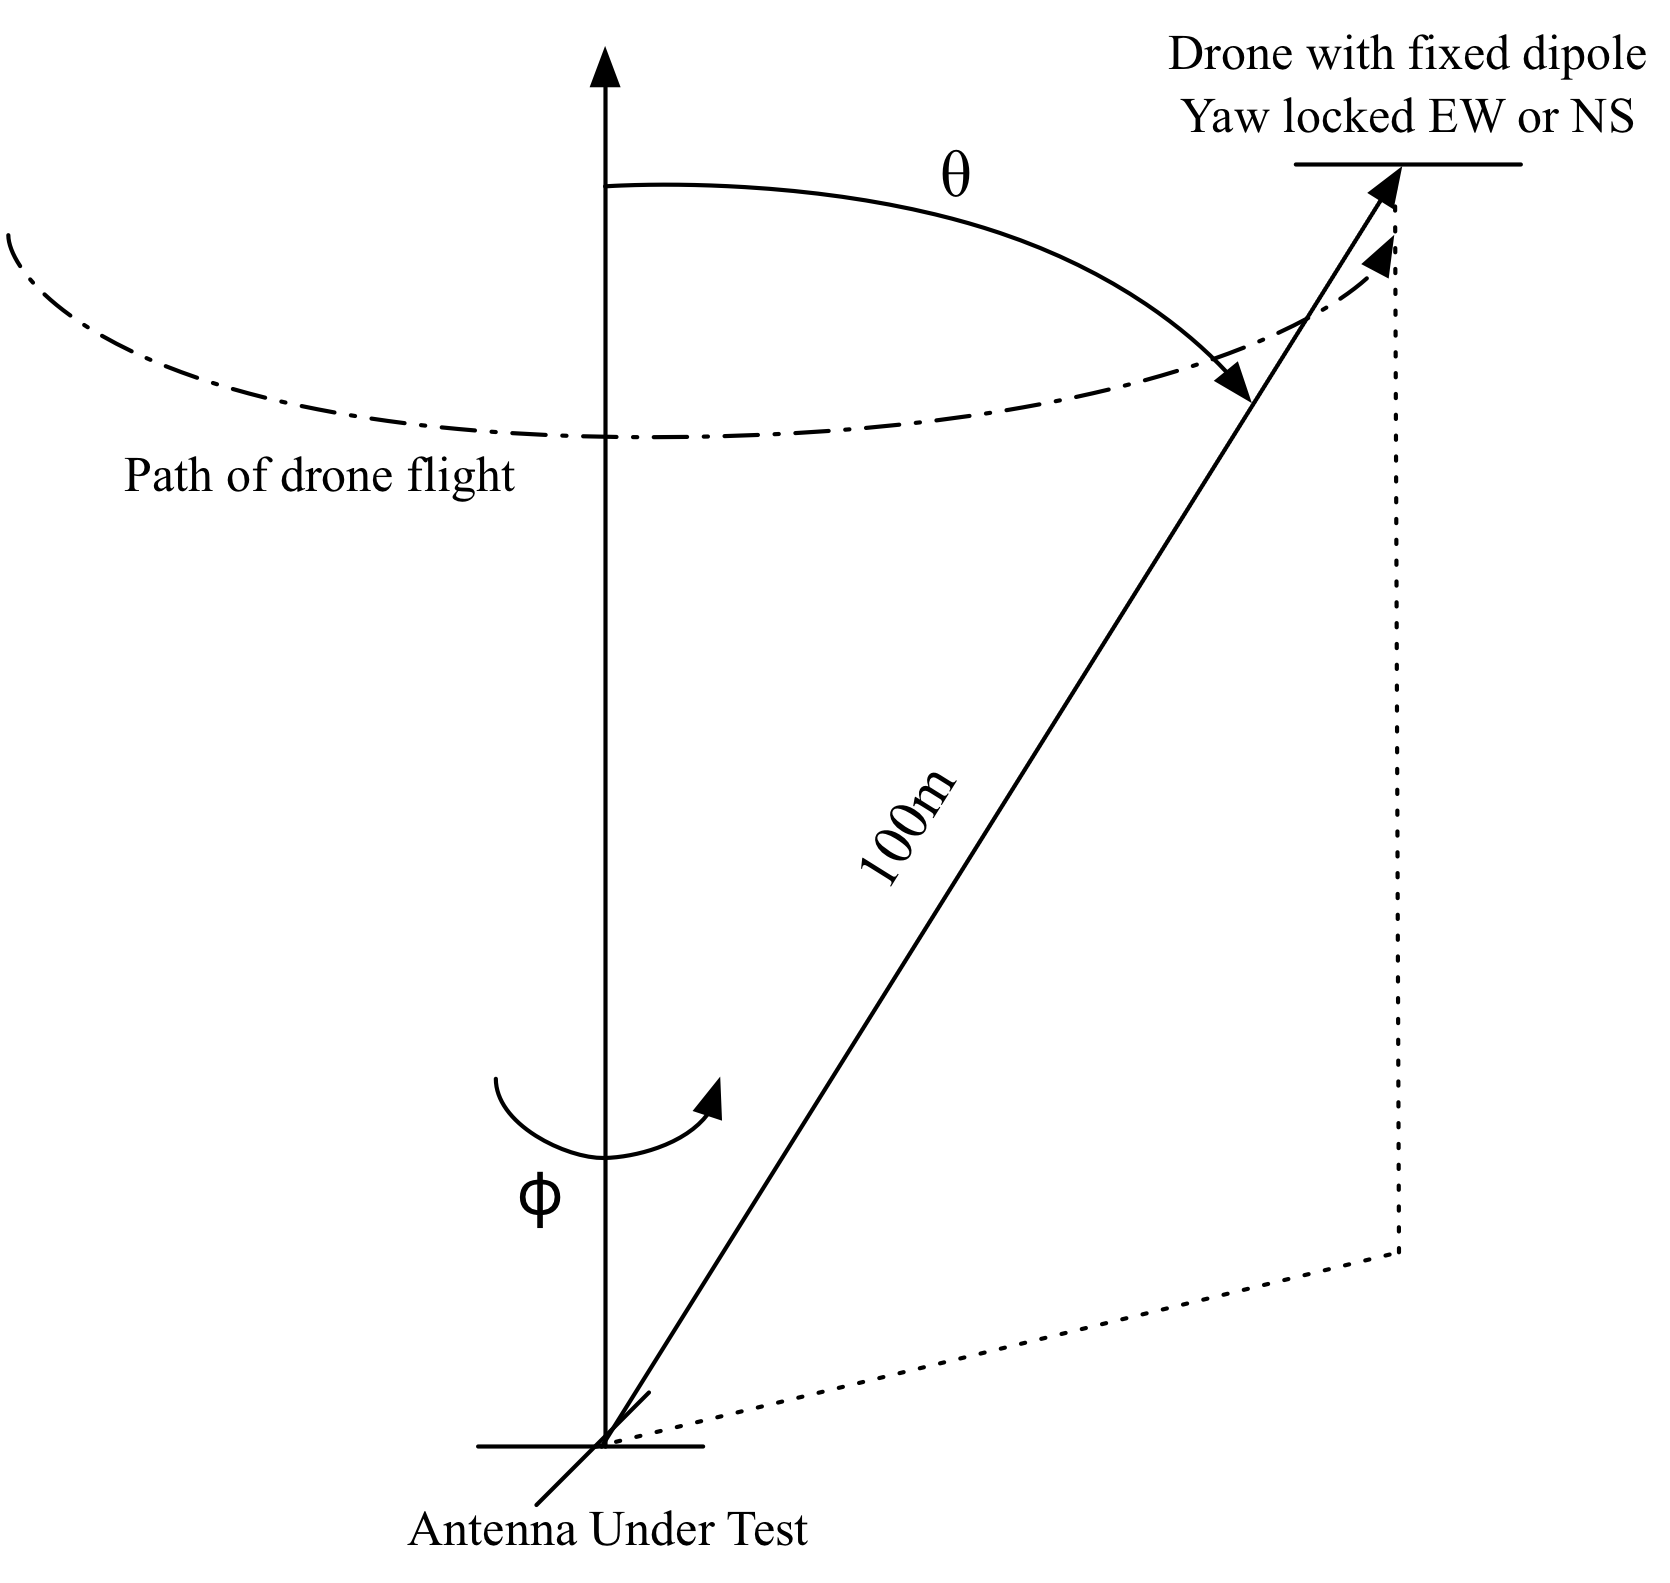
\includegraphics[width=0.6\columnwidth]{figures/ECHO_flight_diagram.png}
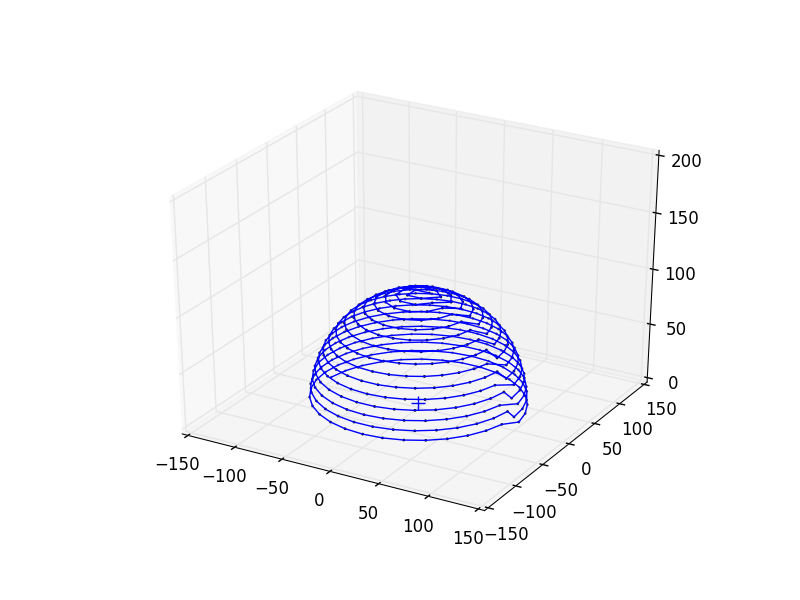
\includegraphics[width=0.39\textwidth]{figures/ECHO_flight_path.png}
\caption{The spherical coordinate system used here relative to the antenna under test (left) and the programmed flight pattern which uses the healpix equal area pixelization to form spherical shell of radius 100m centered on the antenna under test (right). In all flights the dipole antenna is mounted in a fixed position relative to the drone itself so that the drone yaw (rotation about the vertical) controls the transmitter polarization angle. }
\end{center}
\end{figure*}

\section{Design and Method}
\label{sec:design}

\subsection{Drone and Transmitter}
We use an X8 octoquad from 3DRobotics (3DR) with a Pixhawk autopilot running Arducopter 3.5.  With a 10,000 mAh battery and a 1kg payload this setup has a flight time of $\sim$15 minutes. Position is recorded by a Ublox GPS and a barometric altimeter.  The transmitter is a programmable Valon 5007 voltage controlled oscillator. Typically used as a clock signal this device can produce a stable, continuous wave, signal tuned from 137\,MHz to 5\,GHz and is programmable via usb interface.  A continuous wave signal is chosen over a broadband signal for our first testing because the power is concentrated in a narrow band and does not require additional amplification. This reduces both weight and complexity and enables better flexibility to avoid interference.  In the work reported here the transmitter is programmed to broadcast at 137.5\,MHz with attenuation added to produce -25dBm of output power chosen to reach a peak SNR of 40dB without evidence of saturation in the receiver.  The transmit antenna is a BicoLOG 30100 biconical antenna manufactured by Aaronia. It is completely passive, has a smooth spectral response, an operational spectral range of 20\,MHz to 3\,GHz and is light-weight yet robust. 



\subsection{Antenna Mount}
The antenna mounting is chosen to maximize the distance from the drone while preserving stability. The X8 drone legs are too short to permit a fixed mounting further than two or three centimeters below the drone and the wingspan is too narrow for safe landing on longer legs. In the tests here the antenna has been suspended from the drone legs by non-conductive monofilament with a plastic bracket providing the filament/antenna mount point. On the ground, the antenna fits between the legs, in the air the antenna hangs 30\,cm below, this is shown in Figure \ref{fig:drone}. The advantages of this system are that it is simple, extremely light-weight and provides isolation between drone and antenna. The disadvantages are that it lacks rigidity, stability, and because it must be re-tied after transport it is difficult to repeat.  In this scheme, with the antenna fixed in position relative to the drone, the drone yaw (rotation about the vertical) controls the transmitter polarization angle. 

\subsection{Flight Path}
One of the main difficulties encountered by \citet{2015PASP..127.1131C} was in matching the flight pattern to the size scale of the variation in the beam.  They chose a cartesian grid pattern with a separation such that the drone passed through the primary lobe roughly three times.  When combined with the on/off switching used to subtract the 1GHz noise of the drone motors, the number density of samples became extremely limited and led to spurious results when interpolating to make a complete beam map.  Here our goal is to smoothly map the beam of a very wide-field element from zenith to the horizon, which would be difficult with a constant altitude flight pattern.  This is also true of the analysis pipelines where the distortion caused by the gnomic projection to a tangent plane makes for a poor gridding scheme at the horizon. In many 21cm pipelines, the HEALPix pixelization scheme \citep{Gorski:2005p7667} is used to store images and beam models.  HEALPix divides the sky into equal area pixels with the pixel count and resolution selectable by powers of two.

\begin{figure}[htb]
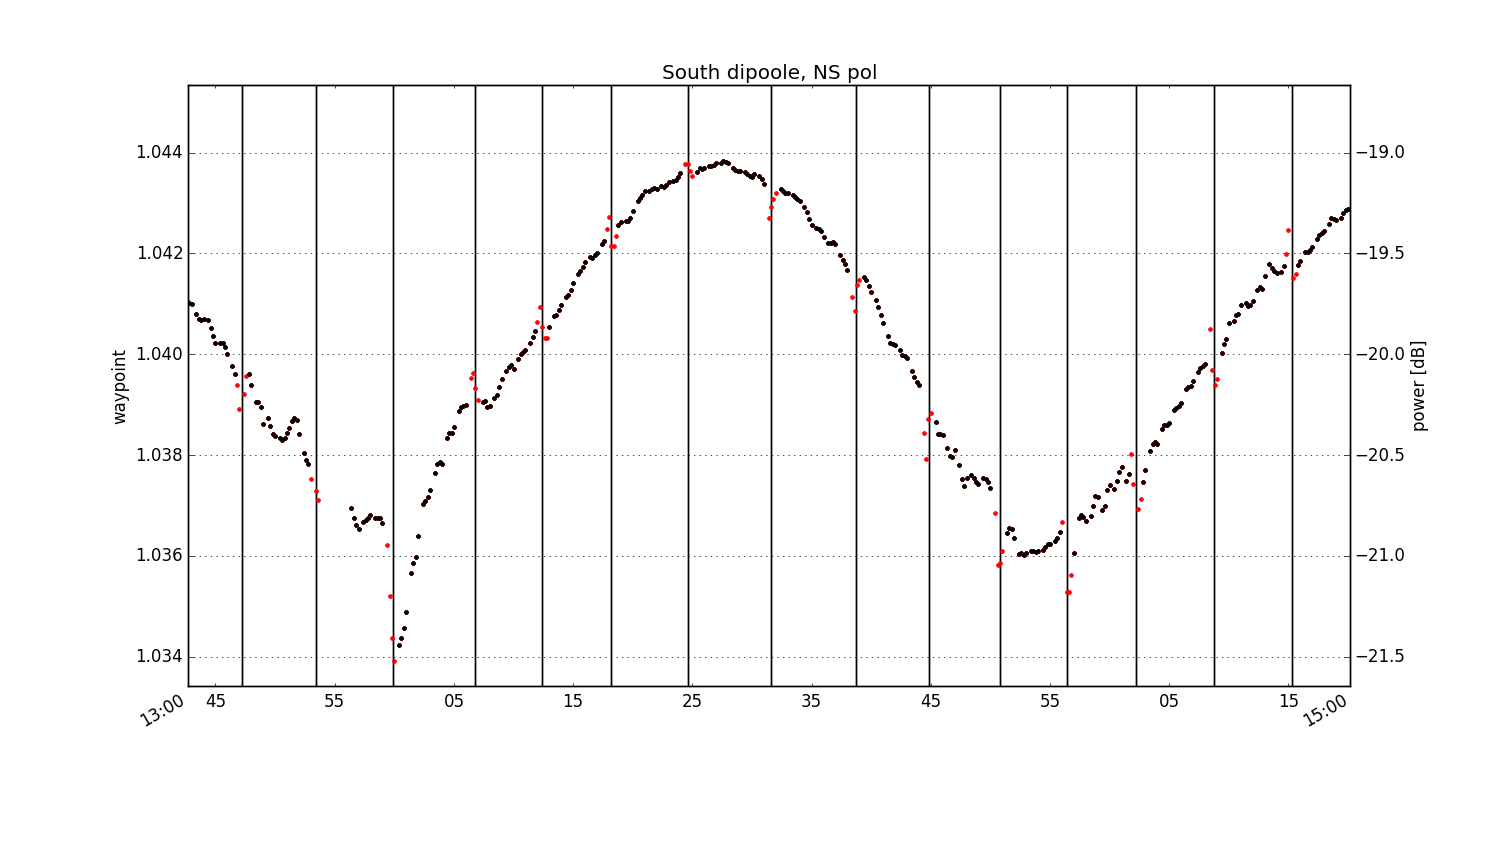
\includegraphics[width=\columnwidth]{figures/GB_waypoint_flagging_zoom.png}
\caption{Received power as a function of time. The drone is observed to shudder slightly when it goes through waypoints (vertical lines) an effect visible in the received power. Here we flag received data within half a second of a waypoint arrival (points in red).}
\label{fig:waypoint_flagging}
\end{figure}

\begin{figure*}[ht]
\begin{center}
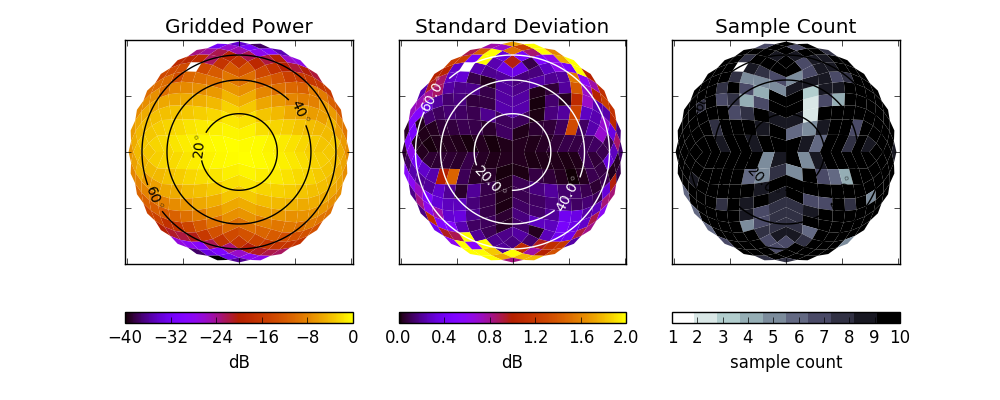
\includegraphics[width=\textwidth]{figures/GB_power_rms_count.png}
\caption{Received power pattern, error, and sample count for a calibration dipole. The received power pattern is shown in its raw form; the beam of the transmitter has not been subtracted.}
\label{fig:beam_std_count}
\end{center}
\end{figure*}
Pixels can be ordered either by their position in the hierarchical doubling (NEST) or in a spiral order with  longitude $\phi$ fastest (RING).  Here we chose a flight pattern which follows the NEST pattern to give us spherical shell flight pattern centered on the receiving antenna with chosen a radius. Following a conservative safety practice limiting to good line of sight and considering the FAA flight ceiling of 400 ft we set the radius (and thus the maximum altitude) to 100m (328ft). The NSIDE parameter sets the number of waypoints and, effectively, the resolution of the beam sampling.  This number is constrained, ultimately by the amount of time available to create a beam map; at constant speed, a denser grid will take longer to record.  The slowest variable to be sampled is GPS position at 2 Hz. We've chosen to fly at 1m/s where the drone will sample about 3 samples per angular degree and an NSIDE of 8.  At this resolution and speed the full $2\pi$ steradians can be mapped to a resolution of 9 degrees in 60 minutes with four 15 minute sorties.

The polarization of the antenna is kept fixed by inserting a Region of Interest (ROI) command into the beginning of the waypoint program.  The ROI command causes the drone to maintain a fixed heading in the direction of a set location which we choose to be a distant location due East or North to match the polarization of the antenna being mapped.


\subsection{Receiver}
Data was collected using the spectrometer setup of the Orbcomm satellite mapping array as described in section 2.4 of \citet{2016:NebenHERAdish}. The software was modified to allow real time inspection of the data, but otherwise the system was operated just as it was for satellite mapping with spectra recorded simultaneously from two dual polarization dipoles at a time cadence of 4 Hz and a spectral resolution of 2kHz. 
\subsection{Data processing}
\label{sec:processing}
We generate a beam map by interpolating the power trace at times when recorded GPS positions are available.  Careful observation of the autopilot behavior and inspection of logs suggests that the X8/Arducopter combination suffers from occasional stability `hiccups'. Finding that these are characterized primarily by outliers in the yaw we have flagged points greater than 2 $\sigma$ above the mean yaw.  Another slight yaw outlier is observed to occur as the drone passes through each waypoint gate which is often accompanied by a visible bump in the received power trace; points within half a second of each waypoint have been flagged (see Figure \ref{fig:waypoint_flagging}).

\begin{figure}
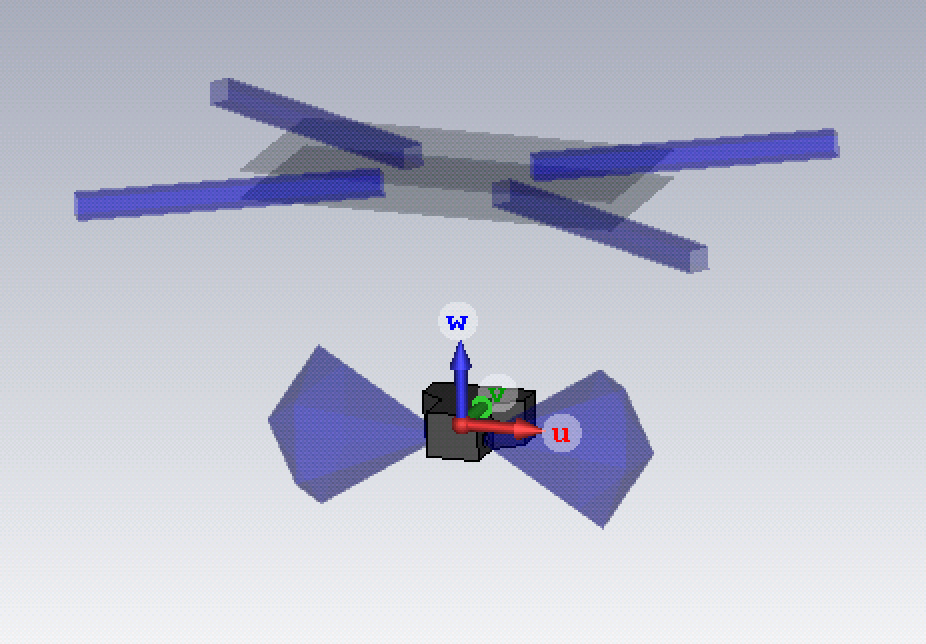
\includegraphics[width=\columnwidth]{figures/drone_antenna_screenshot.png}
\caption{A view of the CST model of the transmitting antenna suspended beneath the metal arms of the drone. The central body, shown in transparent black, is made of non-conductive materials. The largest metallic objects not modeled are the battery which is mounted beneath the central core, the motors on the ends of the arms, and the electronics mounted above the central body.}\label{fig:tx_cst}
\end{figure}




\begin{figure}
\begin{center}
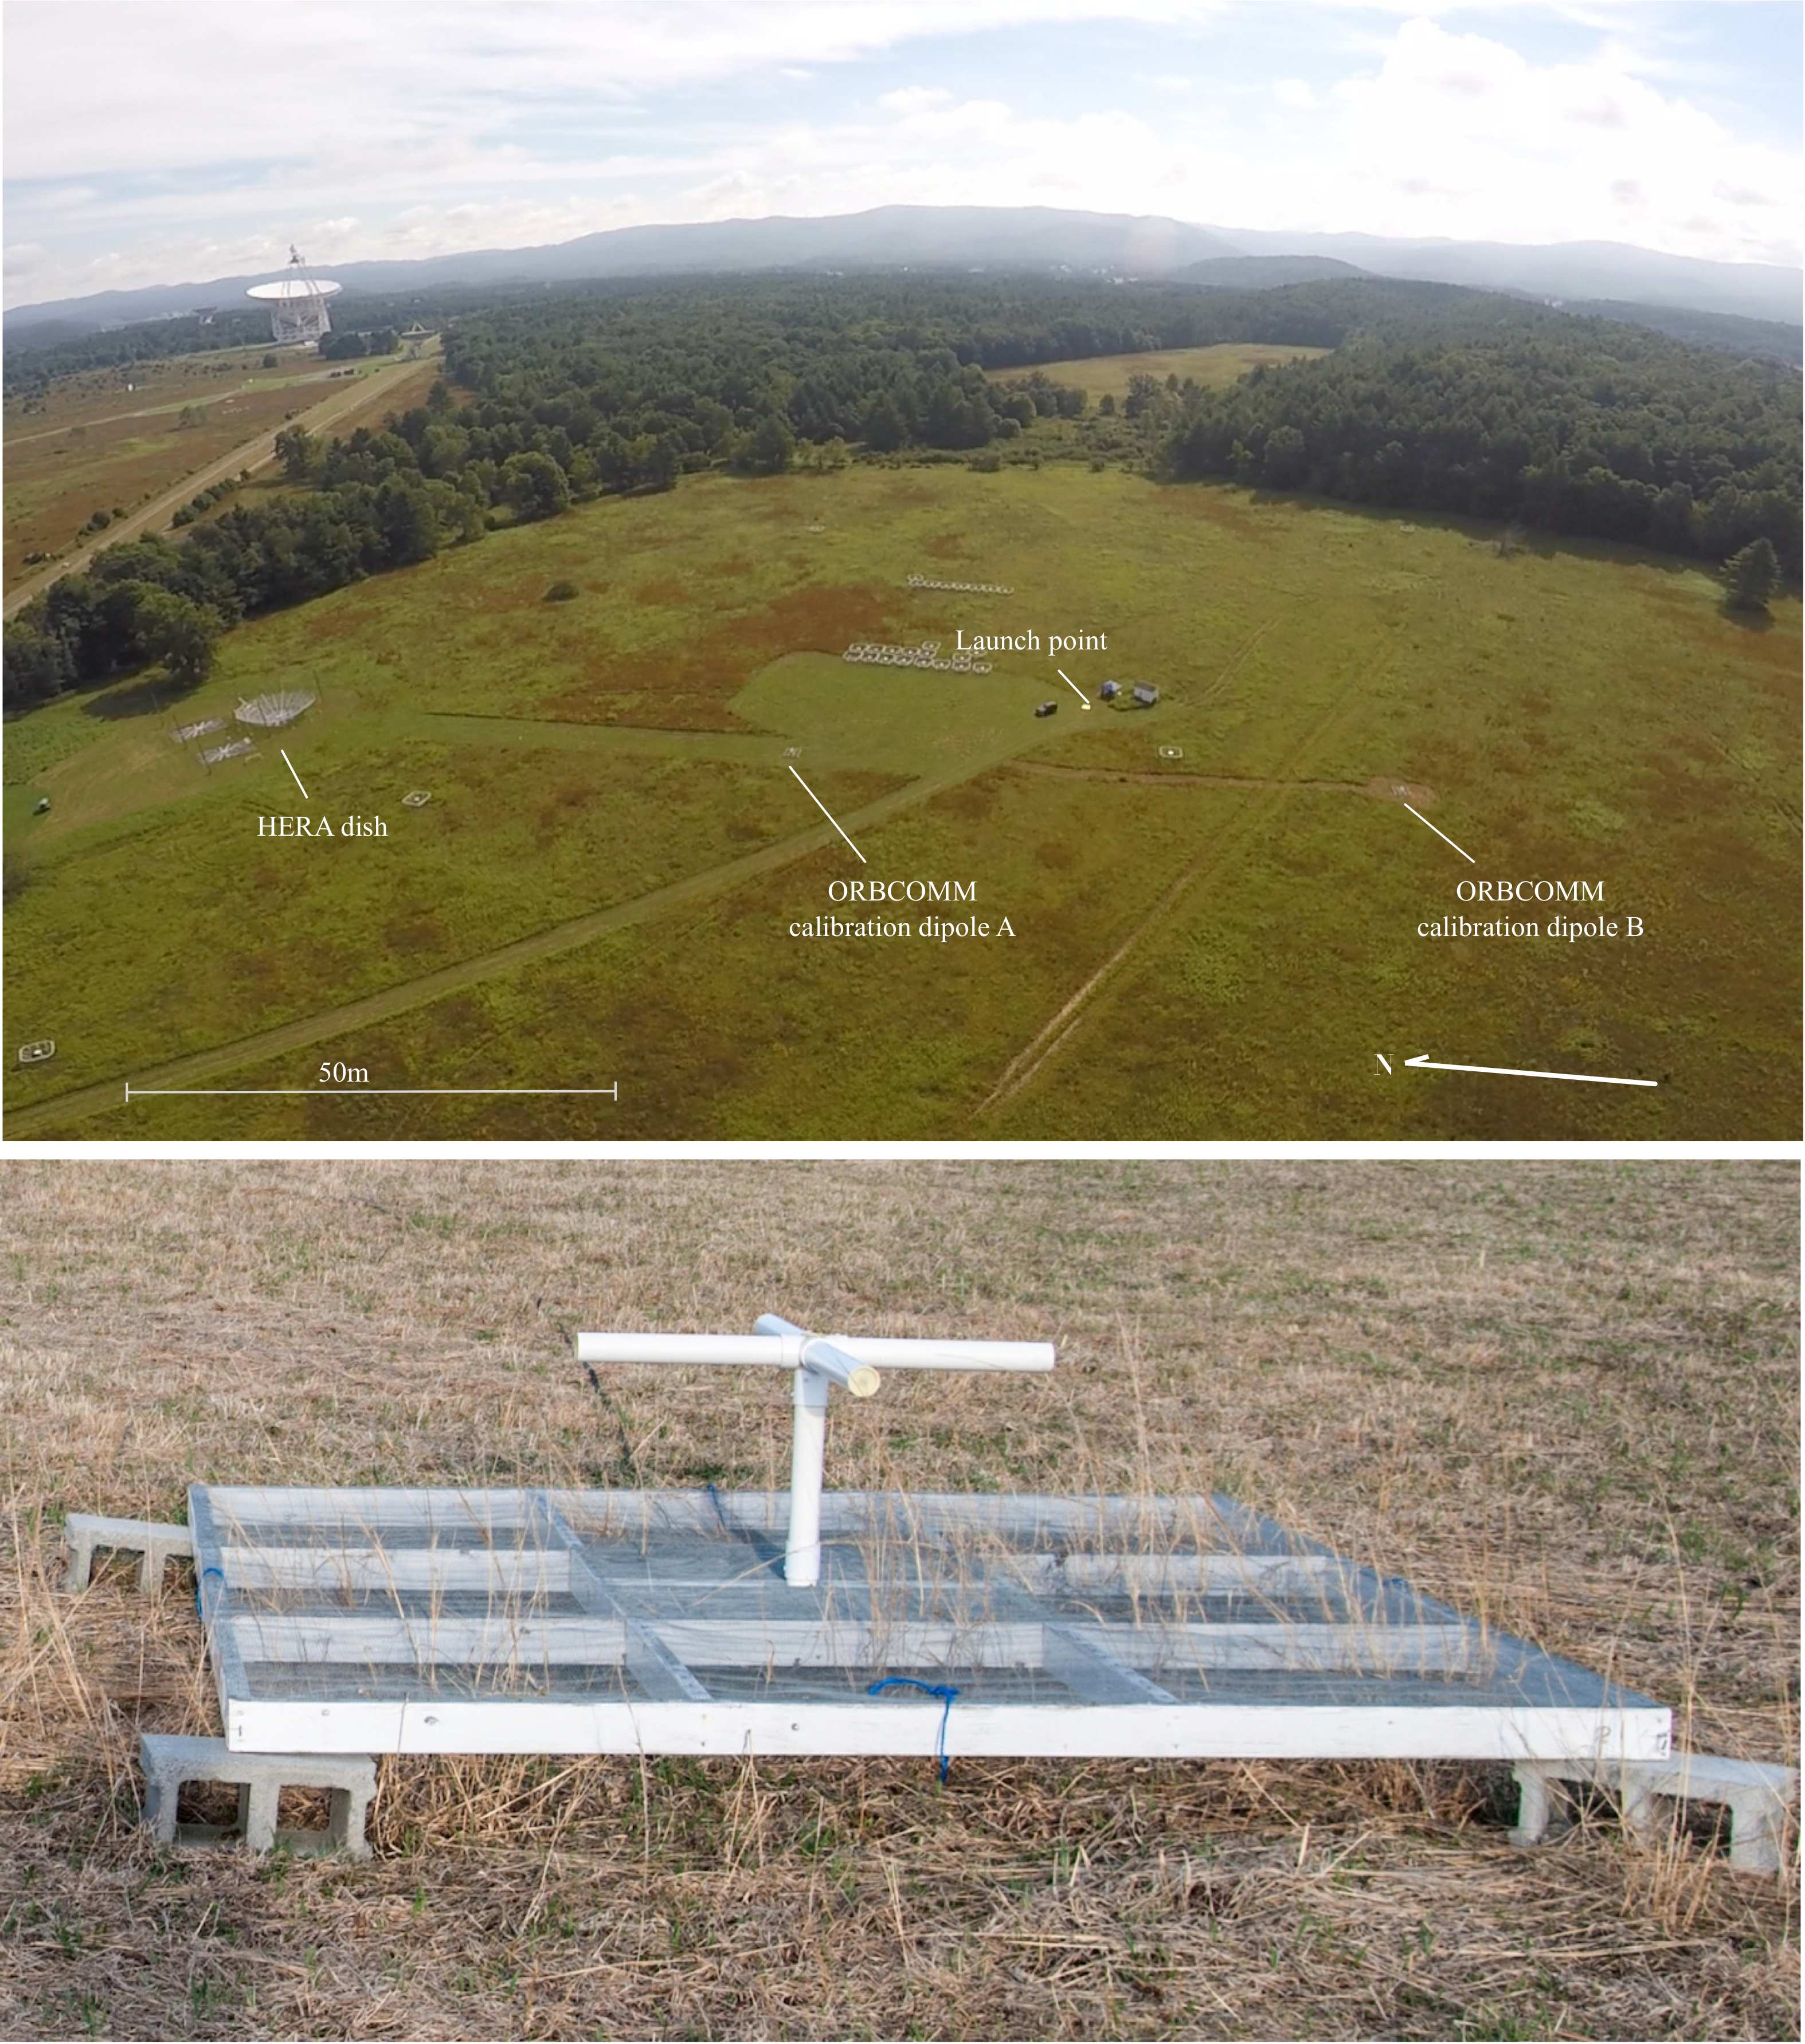
\includegraphics[width=\columnwidth]{figures/Green_Bank_aerial_diagram_extended.png}
\caption{At top, an aerial view of the Orbcomm experimental setup in Green Bank where two calibration stations are separated by 100m on a north south line, as diagrammed on the right. Each calibration station is a dual polarization linear feed mounted on a 2m x 2m mesh set $\sim$20cm above the ground. The spherical flight pattern is centered on each at a radius of 100m.}
\label{fig:GB_aerial}
\end{center}
\end{figure}
%TODO photo of calibration dipole


These flagged data are then gridded, using a nearest pixel approach, into a healpix grid using an NSIDE of 8, the same as the flight pattern.  The gridder records the mean, the standard deviation and the total sample count of all the samples falling into each pixel. An example gridded beam is shown in Figure \ref{fig:beam_std_count}.

The measured power pattern is a product of the power patterns of the transmitter and receiver. To remove the effect of the transmitter beam we divide out a simulation of the beam of the done plus antenna which we model in CST Microwave Studio . The model, shown in Figure \ref{fig:tx_cst} includes the biconical transmitter antenna and the metal arms of the drone; the central body is made of plastic and carbon fiber.  
%, in logarithm this can be written
%\begin{eqnarray*}
% \textrm{tx power} \\
%+ \textrm{tx beam} \\
%+ \textrm{rx beam}\\
%=\textrm{measured power pattern} 
%\end{eqnarray*}

  




\section{Data}
As a first test of stability and accuracy we used ECHO to map antennas which had already been mapped using the Orbcomm satellite constellation.  The Orbcomm system measures the power received from multiple satellites, operating in narrow band channels near 137 MHz and uses the telemetry in those signals to associate the received channel powers with the orbital positions of the satellites \citep{2015RaSc...50..614N}.   The time variation of the digital signal is removed by simultaneously measuring the power received by the antenna under test (AUT) and a nearby, dual polarization, sleeved dipole; the ratio between these two is insensitive to satellite transmitter variations. The reference dipole acts as a precision calibration element and can be calibrated out using a simple model.  The accuracy and repeatability of this scheme can be established with a ``null'' test where the AUT is replaced with a second identical calibration dipole.  The system was in this configuration, in preparation for mapping the HERA beam \citep{Neben2016_HERAOrbcomm}, when we performed the tests described here.  

The setup is shown in Figure \ref{fig:GB_aerial}.  Each calibration station is a dual polarization sleeved dipole mounted over a 4m x 4m mesh screen.  The two stations are separated by 100m along a north south line. In an attempt to minimize confusion we will refer to the north and south stations as A and B, and the relevant polarizations as east-west (EW) and north-south (NS).


Data were collected in a series of four mapping runs in August, 2015 using the Orbcomm setup at the Green Bank Observatory\footnote{The Green Bank Observatory \emph{was} operated by the National Radio Astronomy Observatory which is a facility of the National Science Foundation operated under cooperative agreement by Associated Universities, Inc.}.  The amplifier and receiver setup was left unchanged from normal Orbcomm operations with the exception that the data recording script was modified to increase the spectral dump rate. The ECHO transmitter was tuned to 137.5\,MHz and attenuation was added until, at an output power of -22dBm, saturation into adjacent channels was no longer visible.  This resulted in a signal of amplitude similar to the received -10dB Orbcomm signals. Historical recordings were examined and this channel was seen to be rarely used by Orbcomm making an overlap unlikely.  The output was monitored throughout operations for obvious signs of an overlapping Orbcomm transmission.

The null experiment, shown in an aerial view in Figure \ref{fig:GB_aerial}, was set up with the antennas separated by 100m along a north-south line.  Each station was mapped twice, once with the transmitter fixed in the east-west (EW) direction and once north-south (NS).  The resulting four data sets were flagged and gridded as described in section \ref{sec:processing}, a representative map is shown in Figure \ref{fig:beam_std_count}. 

%Spend some time describing the map in Figure 4.  Does it look like a dipole?  How much does it fall off, can you see the null, how large is the RMS, how many samples per pixel is typical, etc.
In the Figure \ref{fig:beam_std_count} map we can see the basic features of a dipole oriented North-South; a nearly uniform response along the east-west direction and deep nulls to the north and south.  In the nulls the amplitude reaches -40dB at 70\arcdeg{} from the zenith.  The error is largest near the nulls, topping out at 2dB.


\subsection{Comparison with Orbcomm}
\label{sec:orbcomm}
In the Orbcomm null test, because both sleeved dipoles are measured simultaneously,  the ratio of the beams is actively suppressing the largest source of systematic error, time variation of the Orbcomm signals. However in our case, since data are collected sequentially, one map after another, the ratio can expose experimental systematic errors as well as those due to noise or short term variability.

Assuming the transmitter beam is unchanging between mapping runs, the ratios of the two matching NS and EW elements can be directly compared to data collected nearly simultaneously during an Orbcomm null test.   Doing so we find that the EW dipoles have ratios similar to the Orbcomm measurement, but the NS ratio displays a systematic slope in the NS direction, see Figure \ref{fig:GB_NS_ratio_uncalibrated}
\begin{figure}
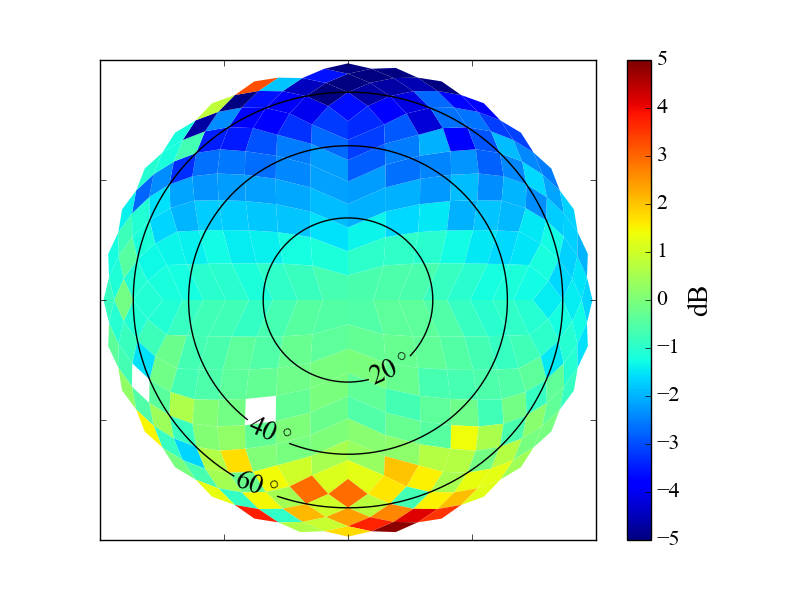
\includegraphics[width=\columnwidth]{figures/GB_NS_ratio_uncalibrated.png}
\caption{The ratio of the two North/South polarization dipoles is expected to be largely unity and to reveal measurement errors. Here we see the presence of a strong north/south gradient which has been identified with a 10\arcdeg{} title of the transmitting antenna during the north map run. See Fig \ref{fig:GB_ratio_maps} where this has been corrected. }\label{fig:GB_NS_ratio_uncalibrated}
\end{figure}


\begin{figure*}
\begin{minipage}{0.45\textwidth}
\centering
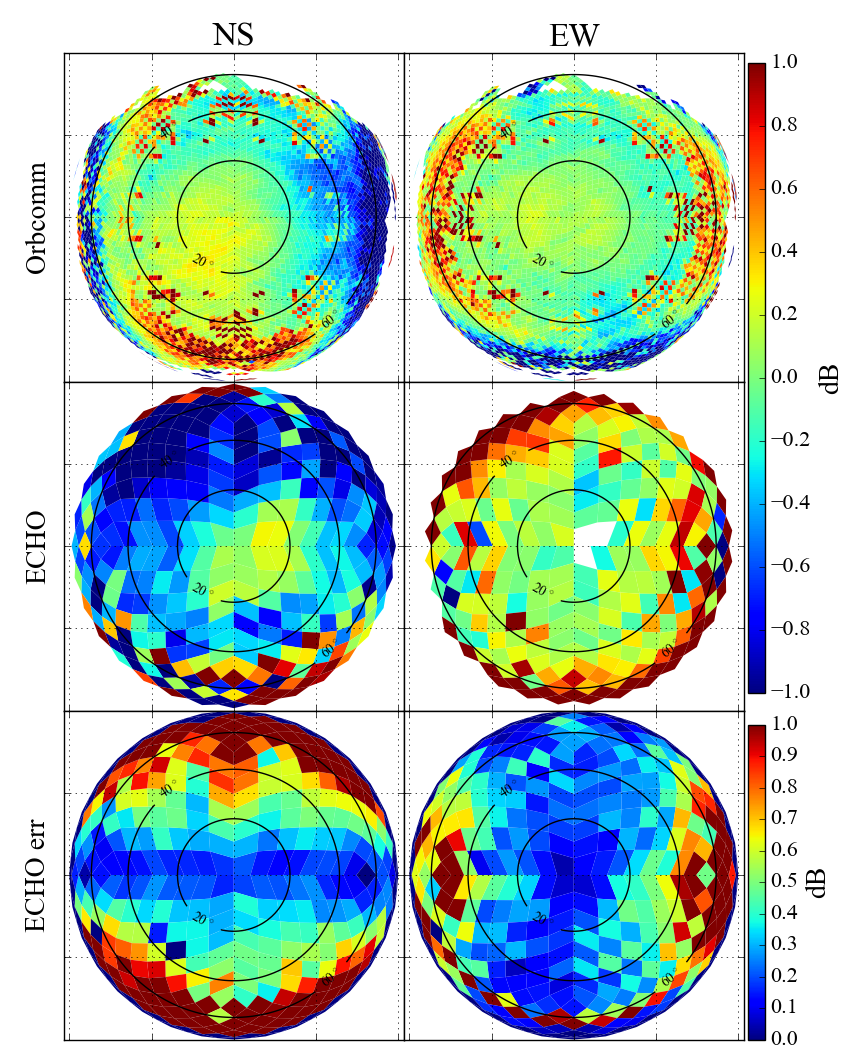
\includegraphics[width=\textwidth]{figures/GB_OC_ratio_compare.png}
\caption{Power pattern ratios between null experiment dipoles compared against similar measurements made with the Orbcomm satellite system (top).  Both methods agree that the EW dipoles are more alike than the NS, though disagree on nature and extent of the difference.  The bottom panels show the standard deviation of the samples within each pixel. The error is smallest in the H plane and increases towards the nulls, this is consistent with $\sim$ degree scale rotation instability in the drone-mounted antenna.}\label{fig:GB_ratio_maps}
\end{minipage}
\centering
\begin{minipage}{0.45\textwidth}
\centering
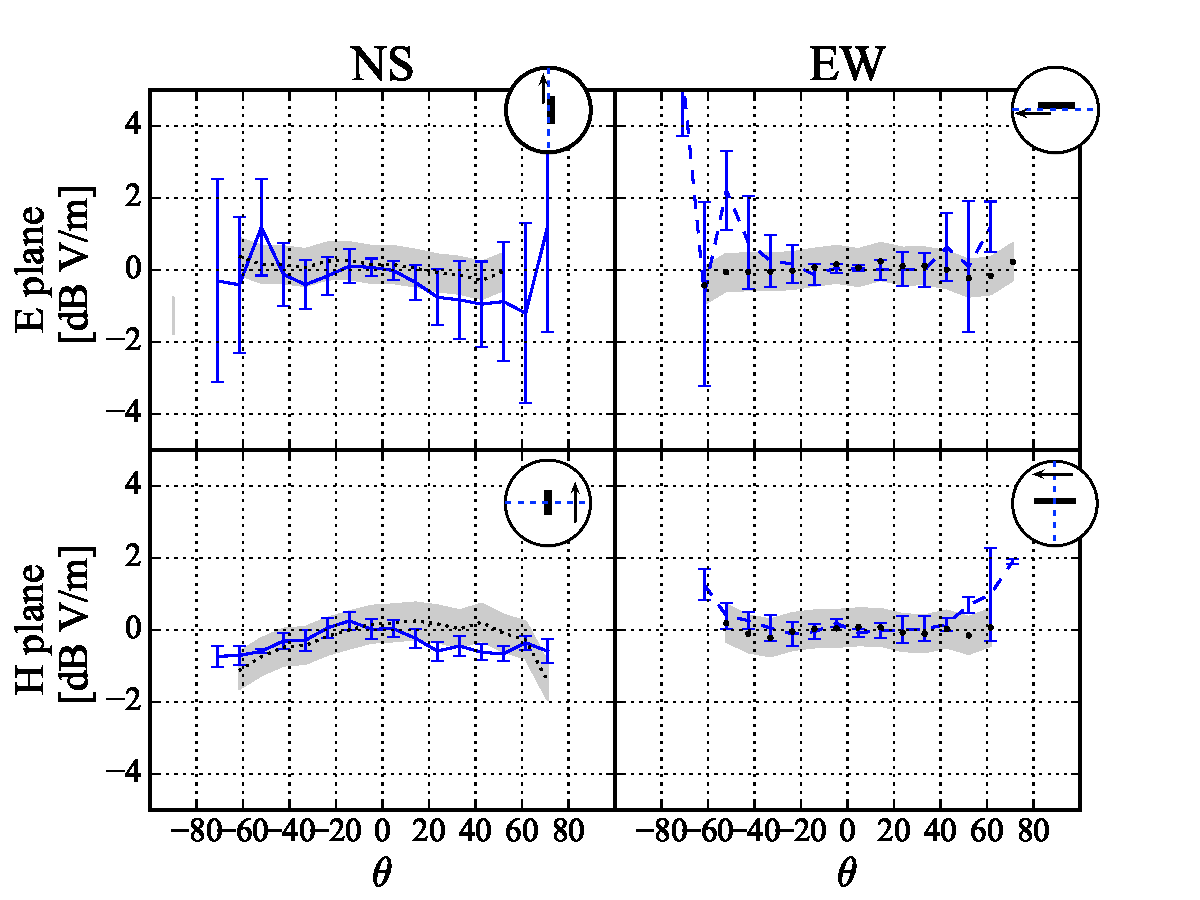
\includegraphics[width=\columnwidth]{figures/GB_ratio_slice_5dB.pdf}
\caption{Cross-sections of the ratio between calibration dipoles measured by Orbcomm (grey) and ECHO (blue).    The little circular glyph indicates polarization and slice geometry: the receiving antenna is a thick line, the transmitter is a thin arrow and blue dotted line shows the slice.  Assuming perfectly identical receiver antennas, this ratio would be unity (0 dB). Here we see deviations generally on the scale of the error bars. Errors are larger in the E plane where the dipoles are aligned on their nulls and small rotations can cause larger \label{fig:GB_ratio_slices}}
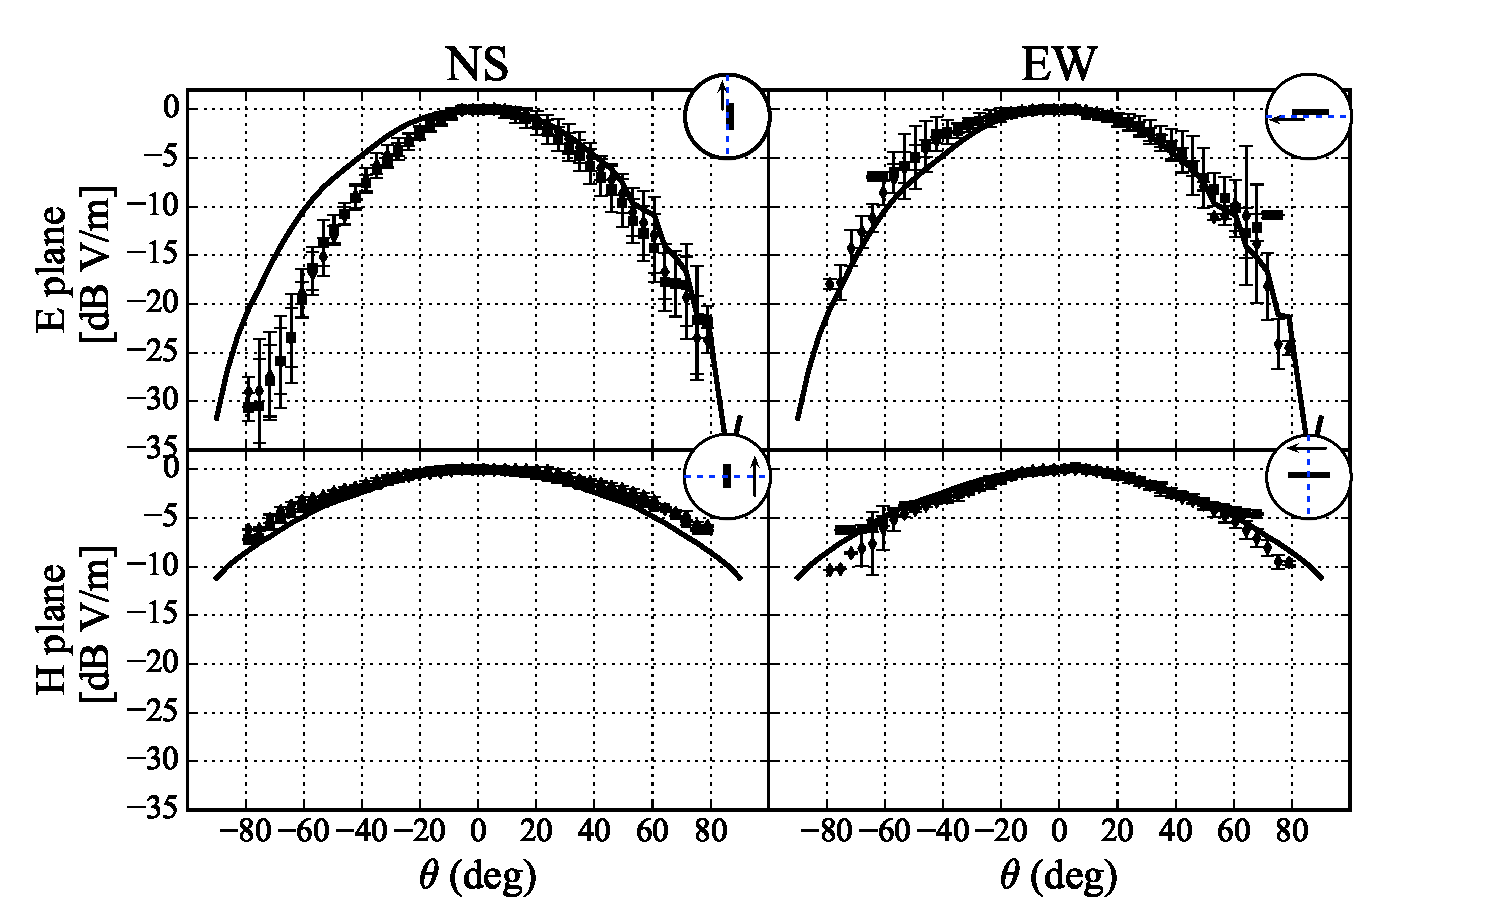
\includegraphics[width=\columnwidth]{figures/GB_slices_quad.pdf}
\caption{Cross-sections of dipole maps after normalizing by transmitter beam pattern. Antenna 'A' is square symbols, antenna 'B' is diamonds and the CST model as solid black. Though both A and B have the same measured beam map to within error bars, they do not always agree with the model. This suggests that the dual polarization feed model might not fully capture the antenna as built.   }\label{fig:GB_slices_quad}
\end{minipage}\hfill
\end{figure*}



Such a slope, aligned with the polarization of the transmitter, can be produced by a modest tilt in the transmitting or receiving antenna. Such a tilt is the most common failure mode of the monofilament transmitter suspension method. If unchanged during the mapping run the tilt can be accounted for by correcting the rotated transmitter beam.  Inspection of photos taken during the field trials revealed several instances of small antenna mounting tilts, most likely in the last mapping run of the experiment, on the NS arm of station A. Here we have, through trial and error, found that a rotation of the transmitter beam by $\Delta \theta = 10$\arcdeg{} provided the best reduction in the slope while staying within the bounds of likely misalignments observed in the field and in the photos. We then went back and re-simulated the transmitter beam in CST with the antenna rotated 10\arcdeg{} with respect to the drone. This rotated transmitter beam model was subtracted from A-NS while an unrotated simulation is subtracted from the other three.

The ratio between the two stations, after subtracting transmitter beams, are plotted in Figures\ref{fig:GB_ratio_maps} and \ref{fig:GB_ratio_slices}.  The slices plotted in Figure \ref{fig:GB_ratio_slices} cut through the E plane parallel to the receiving dipole and the perpendicular H plane.  The E plane cuts through the the dipole nulls and the H plane cuts through the part of the beam with the flattest response.    This geometry is indicated in the figure with a little glyph.

Comparing Figure \ref{fig:GB_NS_ratio_uncalibrated} to the beam-tilt corrected version in Figure \ref{fig:GB_ratio_maps} we can see that 10dB slope across the beam has been reduced to a much smaller difference of around 0.5 dB, which is closer to the scale of the error bars plotted in that same figure. Whether this difference is due to residual antenna orientation miscalibration or is capturing true differences between the identical antennas is difficult to say, however taken at face value, both the Orbcomm and ECHO data agree that the A and B NS polarizations are not as similar to each other as the EW polarizations. Slices of the ratio maps in Figure \ref{fig:GB_ratio_slices} tell a similar story.  The E plane cuts through the nulls of both the receiver and the transmitter tend to reveal the most uncertain portion of the beam. Here the sensitivity is lowest and both beams are a steep function of view angle;  small variations in the orientation of the transmitter can cause large variations in power received within a single healpix pixel.  As we can see in Figure \ref{fig:GB_ratio_slices}, typical measurement error ranges from 1 to 3 dB in the worst case and any systematic deviation from the Orbcomm measurements is typically consistent with these error bars. 

In percentage terms the best measurements are those in the H plane where measurement errors were typically 1\%. These errors were roughly on the same scale as the measured difference between the two antennas as well as the difference between model and data.  Error increased linearly with azimuthal angle and to 6\% in the E plane at low elevation where the two dipoles have their nulls aligned. In this geometry, small rotations of the transmitter antenna can cause large changes in the transmitter beam. Applying a gaussian random rotation to the transmitter beam model, we find that the observed variation is consistent with a rotation RMS of 1.3\arcdeg{}.  This is not far from the observed RMS of the drone yaw is 2.2\arcdeg{}.  The measured yaw is likely to be influenced by other errors such as magnetic interference from the motor currents and is an overestimate of actual drone motion.

\subsection{Comparison to Model}

While the ratio of two identical nearby dipoles provides is a strong test for systematic error, the direct comparison of each measurement against the electromagnetic model is perhaps more diagnostic because we can examine each of the four measurements independently and make direct comparison with the simulated receiver beam. In Figure \ref{fig:GB_slices_quad} we plot orthogonal E and H plane slices of both data and model. The maps of the EW polarization arms seem to agree to within error bars in most places, but while the NS patterns agree with each other to within error bars, they do not agree with the model. 

Nominally we would expect the two polarizations of the dipoles to be identical under 90\arcdeg{} rotations.  The NS arms have deeper nulls and a flatter response along the H plane. Experimenting with a similar rotation fit as was done for the A-NS we found that a simple rotation of the NS arms relative to the EW arms of the receiver dipole cannot account for this difference. Another possibility is unmodeled difference in the construction of the Orbcomm null dipoles.





\section{Conclusion}
\label{sec:conclusion}
In this paper we've described the development and characterization of an airborne radio calibrator specifically targeted at the needs of high-redshift 21cm experiments. The necessity for precision foreground subtraction at one part in 10,000 motivates our desire to make a high fidelity map of the polarized beam response of the as-built antennas. Simulations have shown that beam maps must cover the full $2\pi$ steradians of the sky at uniform precision. 

The design studied here is a relatively simplistic execution with a single dipole fixed beneath a smaller, low cost, commercially available multi-rotor drone.  We tested this design by mapping a set of calibration dipoles for which both data and high fidelity models are available.   From this first trial we draw several conclusions.

\subsection{Mapping Efficiency}
The one previous beam mapping experiment by Chang et al (2015) used a rectilinear grid and found difficulty efficiently sampling the beam with a uniform coverage in a reasonable amount of time.   In that case the AUT was a dish with a fairly narrow field of view coverable with a level flight path. A level rectinilear grid becomes even more problematic when we want to map the wide-field response.  Measuring the response to the horizon would require a very large flight pattern. Given the requirement of sampling the beam over the full half sphere we chose as our flight path the ring pattern Healpix pixelization. This is a signficant advance over regular level grids as it makes possible sampling near to the horizon level without having to fly far away. However, it does not ease the issue of resolution (our maps here were 7\arcdeg{}, for which a denser flight grid is required. Nor sample variance for which a slower flight speed is required. The simplest solution to both issues is more flight time. With a flight lifetime of 15 minutes, each map reported here required 4 flights and with no issues took about 100 minutes; the battery swap overhead is nearly 70\%.  A drone with a 30 minute flight time is possible with currently available technology and would make possible higher resolution maps.

\subsection{Sources of Error}
We found that under most circumstances, the repeatability of multiple measurements of a single beam point had a typical standard deviation of 2\% after flagging on the telemetry data. However we see that the variance increases as transmitter polarization becomes aligned with the receiver (ie in the nulls). In the null of the dipole beam the error was about $\sim$6\%. One possible source of this instability is if the transmitter antenna were rotating in its harness. Turning to our model of the transmitter beam, we see that a yaw RMS of only 1.3\arcdeg{} is sufficient to cause a 6\% error. This error is likely to be a combination of actual yaw instability in the drone and instability of the monofilament mounting method. This kind of instability is typically solved in drone applications by a self-stabilizing gimbal which is commonly used for photography and cinematography. Use of such a thing was avoided in this first iteration to avoid the addition of more conductive components. As this instability is the largest source of error, the benefits from addition of a gimbal  mechanism will likely outweigh the cost of a more complex transmitter beam. 

\subsection{Areas for Improvement}
The sling mounting was chosen under the assumption that distance from the drone would improve the symmetry of the transmitter beam, however subsequent modeling in CST has shown that small changes in distance cause very little beam asymmetry.  Given the instability of the sling method, investigation is currently under way into options for solid mounts closer to the drone body.  Furthermore variance is correlated with excessive yaw (rotation around the vertical). This error is likely to be a combination of actual yaw instability in the drone and instability of the monofilament mounting method. This suggests that we must ensure more stable flight. Care must be taken to shield the magnetometer from the high currents feeding the prop motors and to properly tune the flight control loop settings to yield slow and stable turning.   Finally, for reasons of increased inertia, stability increases with the size of the drone, hence larger drones may be better suited for the application than the one used in this work.

In the end, drone stability can only be refined so far. In most drone applications, this kind of instability is typically solved with a self-stabilizing gimbal which is commonly used for photography and cinematography. Use of such a thing was avoided in this first iteration to minimize weight and to avoid the addition of more conductive components. As this instability is the largest source of error, the benefits from addition of a gimbal mechanism will likely outweigh the costs. 

Comparing our data with the electromagnetic model of the receiver dipole, we found that our data agreed with the model on one of the polarizations, but not the other.  This was true for both identically constructed test stations. As these stations serve as the underlying basis for the accuracy of the drone system, future work should focus on identifying such differences improving the accuracy of our models.

Other areas for further development include extension across the 21cm bands. Coverage of the reionization (100-200\,MHz) and BAO (400-800\,MHz) bands is possible with the current configuration. A larger antenna will be required for the cosmic dawn band 50-100\,MHz.  The maps we obtain here are fully polarized, however they suffer from sensitivity issues at the poles due to our restriction of the dipoles to be parallel with the ground. Transmitter feeds that transmit both polarizations simultaneously and are gimballed to point at the antenna under test are possible, particularly in the sub meter bands, however more simulations are required to understand the limitations and tradeoffs.

\subsection{Overall Performance}
Is the quality of the mapping at the level necessary for precision foreground subtraction?   If we take as a worst-case, the foreground precision requirement to be 10,000:1, then our target precision is 0.01\%, while our current best demonstrated absolute accuracy is $\sim$1\%.  However, we note that the 10,000 number is not well defined, nor is it clear that it flows from the required flux subtraction precision to the accuracy of the beam. \citet{Shaw2015_chimemmodes} have set the limit of .1\% on the width of the beam, which for a gaussian beam translates to $\sim$ 1dB error bars at a -40dB level. Here we have demonstrated 2dB at the -30dB level.  More work is required to both refine the target accuracy, as well as the best way to deliver and verify that accuracy, however it does appear to be very achievable.




\section*{Open Project}
This project is an open-source platform which can be used and modified by anyone. The code used to plan flights and to reduce the data is available at \url{github.com/dannyjacobs/ECHO}; the data in this paper and the plotting scripts are available in this paper's repository \url{github.com/dannyjacobs/ECHO_paper1/}.





\acknowledgments
ECHO development is supported by a grant from the National Science Foundation AST program, award number 1407646. D.C.J would like to acknowledge support by the NSF Astronomy and Astrophysics Fellowship Program under award 1401708.
We thank Rich Bradley and staff at the National Radio Astronomy Observatory, Green Bank and Andri Gretarsson and Embry Riddle Aeronautical Observatory for generously supporting this project with their time and equipment. This project makes use of the Astropy python library \citep{2013Robitaille_Astropy}.

\bibliographystyle{apj}
\bibliography{library}

\end{document}




